\documentclass[oneside,notitlepage,12pt]{article}
\pagestyle{plain}

%\usepackage{polish}
\usepackage[british,UKenglish,USenglish,american]{babel}
\usepackage[utf8]{inputenc}

\usepackage{amssymb}
\usepackage[leqno]{amsmath}
\usepackage{amsfonts}
\usepackage{amsopn}
\usepackage{amstext}
\usepackage{amsthm}
\usepackage[textsize=small]{todonotes}
%\usepackage[disable]{todonotes}
\setuptodonotes{color=blue!30}
\usepackage{enumitem}

\usepackage{tikz}
\usetikzlibrary{cd}

\usepackage{verbatim}
\usepackage[colorlinks, backref, citecolor=blue]{hyperref}
\usepackage[numbers]{natbib}
\usepackage{makeidx}

\newcommand{\define}[2]{{\em #1}\index{#2}}


% Packages for special symbols and ornaments:
\usepackage{calrsfs}
\usepackage{fourier-orns}
%\usepackage{hieroglf} \newcommand{\hiero}{\textpmhg}
\usepackage{clock} %\ClockFrametrue\ClockStyle2
\usepackage[alpine, weather]{ifsym}
\usepackage{tabularx} % extra features for tabular environment
\usepackage{graphicx} % takes care of graphic including machinery
\usepackage{blindtext}
\usepackage{soul}
\usepackage{physics}
\usepackage{qcircuit}
\usepackage{subcaption} 
\usepackage{framed} 

% Resolve rho and varrho symbols
\usepackage{mathptmx}
\DeclareSymbolFont{newfont}{OML}{cmm}{m}{it}% Computer Modern math font
\DeclareMathSymbol{\Epsilon}{3}{newfont}{15}% Symbol 15
\DeclareMathSymbol{\Rho}{\mathalpha}{operators}{"50}

% Formatting page
\usepackage{setspace}

%PAGE SETUP
\textheight=22cm
\textwidth=15cm
%\hoffset=-1cm
\hoffset=1cm
\voffset=-2cm
%\parindent=16pt
\setlength{\marginparwidth}{4cm}
\reversemarginpar

% Notes in margins and switching them on and off (if needed)
\newcommand{\almarginpar}[1]{\leavevmode\marginpar[\raggedleft\small\em{#1}]{}}
%\newcommand{\almarginpar}[1]{}

\providecommand{\ar}{\arrow}
\newcommand{\Em}{\mathbb M}


\frenchspacing

\providecommand{\cal}{\mathcal}
\renewcommand{\Bbb}{\mathbb}
\renewcommand{\frak}{\mathfrak}
\newenvironment{pf}{\begin{proof}}{\end{proof}}

%%%%%%%%%%%%%%%%%%%%
% Standard commands
%%%%%%%%%%%%%%%%%%%%

%%%%%%%%%%%%%%%%%%%%
% Calligraphic and bold letters. 
%%%%%%%%%%%%%%%%%%%%
\newcommand{\Aa}{{\Bbb{A}}}
\newcommand{\Aaa}{{\cal{A}}}
\newcommand{\Bee}{{\cal{B}}}
\newcommand{\Cee}{{\cal{C}}}
\newcommand{\Dee}{{\cal{D}}}
\newcommand{\Ef}{{\cal{F}}}
\newcommand{\Gee}{{\cal{G}}}
\newcommand{\Haa}{{\cal{H}}}
\newcommand{\Ai}{\cal{I}}
\newcommand{\Kay}{{\cal{K}}}
\newcommand{\El}{{\cal{L}}}
\newcommand{\Pee}{{\cal{P}}}
\newcommand{\See}{{\cal{S}}}
\newcommand{\Tau}{{\cal{T}}}
\newcommand{\Yu}{{\cal{U}}}
\newcommand{\Vee}{{\cal{V}}}
\newcommand{\Wu}{{\cal{W}}}
\newcommand{\Zee}{{\Bbb{Z}}}
\newcommand{\Emm}{{\frak{M}}}
\newcommand{\Be}{{\Bbb{B}}}
\newcommand{\Nat}{{\Bbb{N}}}
\newcommand{\Z}{{\mathbb Z}} % The integers
\newcommand{\Qyu}{{\Bbb{Q}}}
\newcommand{\Err}{{\Bbb{R}}}


%%%%%%%%%%%%%%%%%%%%
% Shortcuts for some Greek letters. 
%%%%%%%%%%%%%%%%%%%%
\newcommand{\lam}{{\lambda}}
\newcommand{\al}{\alpha}
\newcommand{\Gam}{\Gamma}
\newcommand{\alG}{\al\in\Gamma}
\newcommand{\sig}{\sigma}
\newcommand{\eps}{\varepsilon}
\renewcommand{\phi}{\varphi}
\renewcommand{\rho}{\varrho}

%%%%%%%%%%%%%%%%%%%%
% Basic commands. 
%%%%%%%%%%%%%%%%%%%%
\newcommand{\rest}{\restriction}
\newcommand{\unii}{\mathbb I}
\newcommand{\ntr}{{n\in\omega}}
\newcommand{\Ntr}{n\in{\Bbb{N}}}
\newcommand{\loe}{\leq}
\newcommand{\goe}{\geq}
\newcommand{\notloe}{\nleq}
\newcommand{\notgoe}{\ngeq}
\newcommand{\subs}{\subseteq}
\newcommand{\sups}{\supseteq}
\newcommand{\nnempty}{\ne\emptyset}
\newcommand{\argum}{\:\cdot\:}
\newcommand{\ovr}{\overline}
\renewcommand{\iff}{\Longleftrightarrow}


%%%%%%%%%%%%%%%%%%%%
% Topology. 
%%%%%%%%%%%%%%%%%%%%
\newcommand{\Cl}[1]{\overline{#1}}
\newcommand{\cl}{\operatorname{cl}}
\newcommand{\Int}{\operatorname{int}}
\newcommand{\w}{\operatorname{w}}
\newcommand{\dens}{\operatorname{dens}}
\newcommand{\eXp}{\operatorname{exp}}
\newcommand{\diam}{\operatorname{diam}}
\newcommand{\dist}{\operatorname{dist}}
\newcommand{\nbd}{\operatorname{nbd}}



%%%%%%%%%%%%%%%%%%%%
% Convexity. 
%%%%%%%%%%%%%%%%%%%%
\newcommand{\conv}{\operatorname{conv}}
\newcommand{\co}{\operatorname{co}}
\newcommand{\clco}{\operatorname{clco}}
\newcommand{\m}{\operatorname{m}}
\newcommand{\med}{\operatorname{med}}

\newcommand{\G}{{\mathbb G}}

%%%%%%%%%%%%%%%%%%%%
% Miscellaneous. 
%%%%%%%%%%%%%%%%%%%%
\newcommand{\id}[1]{{\operatorname{i\!d}_{#1}}} % identity morphism
\newcommand{\cf}{\operatorname{cf}}
\newcommand{\dom}{\operatorname{dom}}
\newcommand{\cod}{\operatorname{cod}}
\newcommand{\Dom}{\operatorname{Dom}}
\newcommand{\rng}{\operatorname{rng}}
\newcommand{\suppt}{\operatorname{suppt}}
\newcommand{\defi}{\stackrel{\rm df}=}
\newcommand{\pr}{\operatorname{pr}}
\newcommand{\liminv}{\varprojlim}

\newcommand{\symd}{\div} % <--- Symmetrical difference

\newcommand{\oraz}{\qquad\text{and}\qquad}

\setcounter{secnumdepth}{5}
\setcounter{tocdepth}{5}
\newcommand\subsubsubsection{\@startsection{paragraph}{4}{\z@}{-2.5ex\@plus -1ex \@minus -.25ex}{1.25ex \@plus .25ex}{\normalfont\normalsize\bfseries}}
\newcommand\subsubsubsubsection{\@startsection{subparagraph}{5}{\z@}{-2.5ex\@plus -1ex \@minus -.25ex}{1.25ex \@plus .25ex}{\normalfont\normalsize\bfseries}}

%%%%%%%%%%%%%%%%%%%%
% Some forcing commands. 
%%%%%%%%%%%%%%%%%%%%
\newcommand{\proves}{\vdash}
\newcommand{\forces}{\Vdash}
\newcommand{\Con}{\operatorname{Con}}
\newcommand{\Card}{{\frak{Card}}}
\newcommand{\Func}{\operatorname{Func}}
\newcommand{\poset}{{\Bbb{P}}}
\newcommand{\Forall}{\forall\;}
\newcommand{\Exists}{\exists\;}
\newcommand{\h}{\widehat}
\newcommand{\val}{\operatorname{val}}
\newcommand{\comp}{\parallel}
\newcommand{\incomp}{\perp}
\newcommand{\Es}{{\cal{S}}}
\newcommand{\meet}{\wedge}
\newcommand{\Meet}{\prod}
\newcommand{\join}{\vee}
\renewcommand{\Join}{\sum}
\newcommand{\Land}{\;\&\;}


%%%%%%%%%%%%%%%%%%%%
% Trees. 
%%%%%%%%%%%%%%%%%%%%
\newcommand{\Lev}{\operatorname{Lev}}
\newcommand{\lev}[2]{{\ell_{#1}#2}}
\newcommand{\Ht}{\operatorname{ht}}
\newcommand{\length}{\operatorname{length}}
\newcommand{\bd}{\partial}

\newcommand{\concat}{{}^\smallfrown}
\newcommand{\Reg}{{\frak{Reg}}}
\newcommand{\Ord}{{\frak{Ord}}}
\newcommand{\by}[1]{/_{#1}}
\newcommand{\club}{\operatorname{club}}
\newcommand{\proj}{\operatorname{proj}}
\newcommand{\otp}{\operatorname{otp}}
\newcommand{\Fin}{\operatorname{fin}}

%%%%%%%%%%%%%%%%%%%%
% Theorems and Propositions. 
%%%%%%%%%%%%%%%%%%%%
\newtheorem{tw}{Theorem}[section]
\newtheorem{wn}[tw]{Corollary}
\newtheorem{lm}[tw]{Lemma}
\newtheorem{prop}[tw]{Proposition}
\newtheorem{claim}[tw]{Claim}
\theoremstyle{definition}
\newtheorem{df}[tw]{Definition}
\newtheorem{ex}[tw]{Example}
\newtheorem{pyt}[tw]{Question}
\newtheorem{question}[tw]{Question}
\theoremstyle{remark}
\newtheorem{uwgi}{Remark}
\renewcommand{\theuwgi}{}

%%%%%%%%%%%%%%
% Create notes
%%%%%%%%%%%%%%
\usepackage{enumitem,amssymb}
\newlist{todolist}{itemize}{2}
\setlist[todolist]{label=$\square$}
\usepackage{pifont}
\newcommand{\cmark}{\ding{51}}%
\newcommand{\xmark}{\ding{55}}%
\newcommand{\done}{\rlap{$\square$}{\raisebox{2pt}{\large\hspace{1pt}\cmark}}%
\hspace{-2.5pt}}
\newcommand{\wontfix}{\rlap{$\square$}{\large\hspace{1pt}\xmark}}

% Cantor's stuff:
\newcommand{\Cantor}{2^\omega}

\hypersetup{
	colorlinks=true,       % false: boxed links; true: colored links
	linkcolor=blue,        % color of internal links
	citecolor=blue,        % color of links to bibliography
	filecolor=magenta,     % color of file links
	urlcolor=blue         
}

%++++++++++++++++++++++++++++++++++++++++

\usepackage{ragged2e}

\title{Variational Quantum Algorithms in Finance}
\author{Thanh Nguyen}
\date{October 2022}

\begin{document}
% \onehalfspacing
% \thispagestyle{empty}
\begin{titlepage}
    
\includegraphics[width=0.25\textwidth]{src/CoverPage/Deakin_Logo.jpeg}
    \begin{center}
        \vspace*{4cm}
        {\LARGE Investigation of Barren Plateaus in Quantum Neural Network Development}
        \vspace{3cm}
        \begin{large}


            \bf Submitted as Honours Dissertation in SIT723/SIT724
            \vspace{1cm}

            \bf \today \\
            T1-2022

            \vspace{3cm}
            \textbf{Thanh Nguyen}\\
            STUDENT ID 218583133 \\
            COURSE - Bachelor of IT Honours (S470)
            \vfill

            \bf \normalsize Supervised by: Prof, Jacob Cybulski\\

        \end{large}
    \end{center}
\end{titlepage}


\maketitle
\begin{abstract}
	\emph{This is a placeholder for the real abstract.}
	\\\\
	{\bf Index Terms ---} Quantum Computing, Quantum Machine Learning, Variational Quantum Algorithms, Barren Plateaus, Python Programming, Qiskit.

\end{abstract}

% \begin{IEEEkeywords}
%     Quantum Computing, Quantum Machine Learning, Variational Quantum Algorithms, Barren Plateaus, Python Programming, Qiskit.
% \end{IEEEkeywords}


\tableofcontents
\pagebreak

\section{Introduction} \label{Sec: Introduction}

\emph{Quantum computing} is the area of research that involves physics, computer science and mathematices.
Theoretically, the computational power of a quantum processor would scale exponentially with the number of qubits, and eventually surpasses the classical computers.
For this reason, many algorithms for quantum computers have been developed to solve problems that are challenging for classical computers, eg. the problems that belong to the non-deterministic polynomial time class \cite{williamsSolvingNPCompleteProblems2011,jiangQuantumAnnealingPrime2018,farhiQuantumApproximateOptimization2014}.
Such algorithms are understood as the unitary matrices to perform operations on qubits' values, and are often represented as \emph{quantum gates} on a \emph{quantum circuit}.

In practical, available quantum hardware are severely constrainted in resourse due to decoherence, and their applications are thus limited.
They are all described as Noisy Intermediate-Scale Quantum (or NISQ) computers \cite{brooksQuantumSupremacyHunt2019}.
In other words, we can expect the technical maturity of nowadays quantum devices are comparable to the first computers one hundred years ago.
At the current stage, all NISQ devices face the issue of precision for gate operations, the lack of fault-tolerance design to handle data integrity in case of decoherence, the limitation in the number of qubits in a processor, and the number of gates allowed for those qubits (the size of the circuit).

An approach such as Variational Quantum Algorithms (VQA) \cite{cerezo2021variational} is used to address this issue, by adopting the machine learning models to produce quantum circuits.
This technique involves the quantum circuits as the machine learning models that can receive trainable parameters, which act as a reusable template.
The classical component of the VQA model can feed and train the trainable parameters with any optimisation algorithm available.

VQA is also the mainstream way to design Quantum Neural Network (QNN) \cite{altaisky2001quantum}since they all share the same structure of classical optimisers and quantum ciurcits.
Typical QNN will have the three traits as pointed out by Schuld et al \cite{schuldQuestQuantumNeural2014}: (1) Initial state can encode the data as binary string; (2) The caculation process is based on Neural Network; (3) The system evolution is based on quantum theory.

\todo{Maybe write about VQE? Some applications of QML in Finance}

In this paper, we review the state of the art of quantum machine learning solutions for application in financial sector, especially Portfolio Optimisation and Portfolio Diversification problems.

% In our discussion we will assume that the readers have some background knowledge of quantum computing, linear algebra, and machine learning.
% To gain such a background knowledge, we recommend the 2020 Qiskit Global Summer School course \cite{2020QiskitGlobal}, which provides some basic mathematics, theories and practices of quantum computing.
% The book by Sutor \cite{sutorDancingQubitsHow2019} also provides the foundations of quantum Computing plus an overview of issues related to the design of current quantum hardware and simulators.
% Finally, the 2021 Qiskit Global Summer School course \cite{2021QiskitGlobal} was focused on the selected aspects of machine learning for quantum devices.
\section{Hybrid Quantum - Classical System} \label{Sec: Hybrid Quantum - Classical System}

This section reviews the structure and underpinning mathematics of hybrid quantum - classical algorithms, eg. VQAs.
Such techniques that involves both quantum and classical components have been proposed to address the limitation of NISQ devices \cite{brooksQuantumSupremacyHunt2019}.
Those restrictions include the lack of fault-tolerance design, the number of the available qubits per processors, and the depth of executable quantum circuits the practical use cases.

In more details, the hybrid techniques such as VQA allows development of \emph{parameterised circuits}, which act as a template and capable of receiving trainable parameters.
Those parameters can be used to sample circuits result iteratively in a quantum processor, and consequently be refined by a classical computer \cite{cerezo_variational_2021}.
In this way, we can rely on a wide range of classical optimisers to find the optimal circuit for a particular problem, as these optimisers only treat the variational circutis as black boxes capable of yielding outputs from inputs and the trainable parameters.



The process of solving a problem using VQAs involves three components: the \textit{training data}, the \textit{ansatzes}, and the \textit{Cost function}.
Consider a problem requires VQA to solve and given the training data, we can first construct a \textit{cost function} $C$.
By minimising the cost function value, we can obtain the optimal sequence of parameters $\theta$.
The variational circuit, called \textit{ansatz}, is the target of our training.
We aim to train the ansatz to so that its cost function $C(\theta)$ reaches the minimum value:
\begin{equation}
    \theta^* = \underset{\theta}{\arg \min} \;C(\theta)
    \label{Eqn: optimize theta with ansatz}
\end{equation}
The cost function $C(\theta)$ is estimated by a quantum computer, while we can select a wide range of classical optimiser to train the parameters $\theta$.
Figure \ref{Fig: VQA diagram} this hybrid architecture and demonstrate the training process in more detail.

% Consider a simple problem that we want to solve using VQA, given access to the training data.
% The first step is to construct a \textit{cost function} $C$ used to search for an optimal set of circuit parameters, which is achieved by minimising the cost function during the training process.
% We can simplify the development of variational circuits by composing the circuit templates called \textit{ansatze}.
% \textit{Ansatz} is the parameterised circuit that depends on a set of parameters $\theta$.
% We aim to train the ansatze by optimising the parameters $\theta$s so that the cost function $C$ reaches its minimum, thus satisfying:
% \begin{equation}
%     \theta^* = \underset{\theta}{\arg \min} \;C(\theta)
%     \label{Eqn: optimize theta with ansatz}
% \end{equation}

% In short, the cost function $C(\theta)$ is calculated using the quantum computer, while the classical optimiser trains the parameters $\theta$. Figure \ref{Fig: VQA diagram} explains the VQA architecture and elaborates its training process in more detail.

\begin{figure}
    \centering
    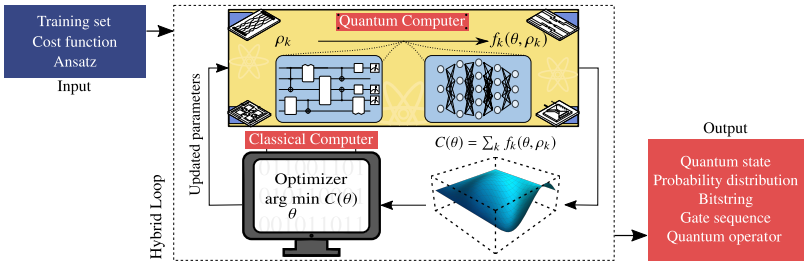
\includegraphics[width=\linewidth]{Appendices/vqadiagram.png}
    \caption{
        An illustrative diagram of a ganeral Variational Quantum Algorithm.
        The algorithm is a hybrid quantum-classical that involves:
        (1) A cost function $C(\theta)$;
        (2) An ansatz that receives trainable parameter $\theta$ and yields outputs from inputs;
        (3) A set of training data $\{\rho_k\}$ so the ansatz can learn the pattern.
        We use the quantum computer to calculate the cost function $C(\theta)$ for each step of optimisation.
        An optimisation algorithm in a classical computer is in charge to find the global minima in the cost landscape of $C(\theta)$, thus satisfy Eq. (\ref{Eqn: optimize theta with ansatz}).
        VQA's result is an approximation of the problem solution, which can be probability distribution, bit string, gate sequence and quantum operator.
        Figure from Cerezo et al. \cite{cerezo_variational_2021}.
    }
    \label{Fig: VQA diagram}
\end{figure}




\subsection{The Cost Function} \label{Sec: The Cost Function}\

% Encoding the problem into a cost function is the first step in solving a problem using VQA \cite{cerezo2021variational}.
% The cost function is equivalent to that used in classical machine learning.
% It maps the values of the trainable parameters $\theta$ into real values, which represent the measure of distance from an optimum solution.
% For a function $f$ that receives input states $\{\rho_k\}$, observables $\{O_k\}$, and a parameterized circuit $U(\theta)$, the cost is expressed as:

Both classical machine learning and quantum machine learning use the cost function to map the the trainable parameters $\theta$ into a value that represent the distance from the optimal solution.
This is the first step in finding a solution using VQA \cite{cerezo2021variational}.
For a function $f$ with the input states $\{\rho_k\}$, the observables $\{O_k\}$ and the parameterised circuit $U(\theta)$, the cost is as following equation:

\begin{equation}
    C(\theta) = f(\{\rho_k\}, \{O_k\}, U(\theta)) \;,
\end{equation}
or this equation with a set of functions $\{f_k\}$ and the trace $Tr$ as the square of a distance matrix:
\begin{equation}
    C(\theta) = \sum_k f_k \left(\Tr[ O_k U(\theta) \rho_k U^\dagger(\theta) ]\right) \;,
    \label{Eqn: Cost function}
\end{equation}

A cost function of an VQA algorithm must meet a number of criteria:
(1) The cost function must be 'faithful' and 'operationally meaningful', the minimum value of $C(\theta)$ should correspond to the optimal solution of the problem, and we can expect the better solution with lower cost function value in general;
(2) The cost function must be 'efficiently estimated' on a quantum computer by measuring qubits values;
(3) The cost function must be 'trainable', such that the parameters $\theta$ could be efficiently optimised.
\subsection{Ansatze} \label{Sec: Ansatze}

\todo{paraphrase}

\begin{figure}
    \centerline{
    \Qcircuit @C=1em @R=0em {
    & \multigate{2}{U_1(\theta_1)}    & \multigate{2}{U_2(\theta_2)}    & \qw &        & & \multigate{2}{U_L(\theta_L)}   & \qw\\
    & \ghost{U_1(\theta_1)}           & \ghost{U_2(\theta_2)}           & \qw & \cdots & & \ghost{U_L(\theta_L)}          & \qw\\
    & \ghost{U_1(\theta_1)}           & \ghost{U_2(\theta_2)}           & \qw &        & & \ghost{U_L(\theta_L)}          & \qw
    \gategroup{1}{2}{3}{7}{.6em}{--}
    }
    }
    \centerline{$U(\theta)$}
    \centerline{}
    \centerline{}
    \centerline{
    \Qcircuit @C=1em @R=0em{
    & \multigate{1}{}   & \ctrl{2}  & \gate{}           & \qw \\
    & \ghost{}          & \qw       & \multigate{1}{}   & \qw \\
    & \gate{}           & \targ     & \ghost{}          & \qw
    \gategroup{1}{2}{3}{4}{.6em}{--}
    }
    }
    \centerline{$U_l(\theta_l)$}
    \caption{
        A diagram of a sample ansatz (above), the ansatz is a sequence of unitaries $U_l(\theta_l)$ (below).
        The ansatz $U(\theta)$ receives parameters $\theta$ is expressed by $L$ layers of unitaries $U_l(\theta_l)$ for $l$ is the layer indices.
        Each unitary $U_l(\theta_l)$ is a circuit composed of a mix of parameterised and unparametrised gates.
    }\label{Fig: Ansatz diagram}
\end{figure}

% In physics and mathematics, \emph{ansatz} (plural \emph{ansatze}) is an educated guess or a starting point from which you start looking for a solution to the problem at hand. 
% In quantum computing, \emph{ansatz} is a parameterised circuit, formed as a sequence of unitary (or "atomic") circuits, which is used as a framework for the circuit optimisation.
% In general, the location of parameters $\theta$ is determined by the ansatz form and can be trained to minimise the cost.
% The ansatz structure can be defined based on the problem (called 'problem-inspired ansatze') or a generic structure (called 'problem agnostic ansatze') that can be used without any relevant information available \cite{cerezo2021variational}.

In physics and mathematics, the term \emph{ansatz} (plural \emph{ansatze}) is reffered to a starting point wich you begin looking for a solution to the problem at hand.
For Quantum computing, we call the parameterised circuit as \emph{ansatz}, form as a sequence of smaller unitary circuits, serves as a framework and the starting point for circuit optimisation.
There are two ways to define the structure of ansatz, we call 'problem-inspired ansatze' if the ansatz is tailor made for a problem, or 'problem agnostic ansatze' for a generic structure that can be used with any problem \cite{cerezo2021variational}.
The location of the parameters $\theta$ in the cost function landscape is determined by the ansatz, and can be further optimised toward the minima.


% The cost function in Eq. (\ref{Eqn: Cost function}) encodes the parameters $\theta$ in a unitary $U(\theta)$ and applies to the input states of the circuit.
% The Figure \ref{Fig: Ansatz diagram} shows that $U(\theta)$ can be expressed as a product of $L$ consecutive unitaries:

The cost function (see Eq. (\ref{Eqn: Cost function})) can encode the parameters $\theta$ in the ansatz $U(\theta)$.
As can be seen from the Figure \ref{Fig: Ansatz diagram}, the ansatz $U(\theta)$ is a chain of consecutive unitaries $U_l(\theta_l)$:
\begin{equation}
    U(\theta) = U_L(\theta_L) \cdots U_2(\theta_2) U_1(\theta_1)\;,
\end{equation}
with each layer of unitary:
\begin{equation}
    U_l(\theta_l) = \prod_m e^{-i\theta_m H_m} W_m
\end{equation}
for unparamaterized unitary $W_m$, hermitian operator $H_m$, and $\theta_l$ is the $l$-th element of $\theta$.
% \subsection{Gradients} \label{Sec: Gradients}
After defining the cost function and a suitable ansatz, we train the parameter $\theta = \{\theta_{l}\}$ to solve the problem in Eq. (\ref{Eqn: optimize theta with ansatz}) \cite{cerezo2021variational}.
The cost function gradient helps the optimiser to find the global minima.
Consider the cost function in Eq. (\ref{Eqn: Cost function}), for a unitary that parameterises rotation $e^{i \theta_l \sigma_{l}}$, where $\theta_l$ be the $l$-th element of $\theta$, $\sigma_l$ is a Pauli rotation operator.
We can evaluate the gradient with the parameter-shift rule:
\begin{equation}
    \frac{\partial C}{\partial\theta_l}
    = \sum_k \frac{1}{2 \sin{\alpha}}
    \left(
    \Tr[O_k U^\dagger(\theta_+) \rho_k U(\theta_+)]
    - \Tr[O_k U^\dagger(\theta_-) \rho_k U(\theta_-)]
    \right) \;,
    \label{Eqn: Parameter-shift rules}
\end{equation}
with $\theta_{\pm} = \theta \pm \alpha e_l$, $\alpha \in \mathbb{R}$ and $e_l$ is a vector such that its $l$-th position have the value of 1, or else 0.

Essentially, we can shift the $l$-th parameter by some amount $\alpha$, and Eq. (\ref{Eqn: Parameter-shift rules}) will calculate the gradient.

\subsection{Optimisers} \label{Sec: Optimisers}
The accuracy of VQA greatly depends on the optimisation method.
Typically, we can achieve the solution by making successive moves along the gradient direction.
This optimisation approach is within the scope of stochastic gradient descent (SGD).
One example of SGD is the ADAM optimiser \cite{kingmaAdamMethodStochastic2014}, which can vary the size of the steps taken during optimisation to produce more efficient and precise results compared to the basic SGD.
\begin{framed}
	Add the following topics:
	\begin{itemize}
		\item Portfolio Optimisation
		\item Price/Option Prediction
		\item Fraud Indicators
		\item Credit Scoring
		\item Financial Risk Assessment
	\end{itemize}
\end{framed}


\section{Portfolio Optimisation - Mean Variance Analysis} \label{Sec: Portfolio Optimisation}

\emph{Portfolio Optimisation} is the problem of optimising the distribution of assets in a period of time to increase the maximum expected returns and minimise any financial risks of the portfolio owners at the end of the trading period \cite{abdelazizMultiobjectiveStochasticProgramming2007}.
By solving the portfolio optimisation problem, owners can achieve risk-free investment, at the same time their long-term profit with the focused on maximise the earnings.

In more detail, for $N$ number of assets, we expect an $N$-dimensional vector of weights $\bar{\omega_t}$.
The weight of each asset $n$ at a peropid time $t = t_i, t_{i+1}, \cdots, t_f$ is $\bar{\omega_{n,t}}$ where $t_i$ is the initial trading time and $t_f$ is the final trading.
$\Sigma_t$ is a $N \times N$ matrix which represents the assets' covariance at time $t$ and $\mu_t$ is $N$-length vector that forcasts the return at time $t$.
For a trading trajectory as a set of vectors $\{ \bar\omega_{t_i}, \cdots, \bar\omega_{t_f} \}$, we estimate the return as following equation:
\begin{equation}
    \text{Return} = \sum^{t_f}_{t=t_i}\mu^T_t \bar\omega_t,
\end{equation}
and the risk of the trading trajectory as:
\begin{equation}
    \text{Risk} = \frac{1}{2} \sum^{t_f}_{t=t_i} \bar\omega^T_t \Sigma_t \bar\omega_t,
\end{equation}

In portfolio optimisation, we aim to find the trajectory that maximise the returns while not raising the risk factor.
We define the total investment $K$ as
\begin{equation} \label{Eqn: normalised weight portfolio}
    \sum^N_{n=1} \bar\omega_{n,t} =  K \forall t,
\end{equation}
and the normalised weight as percentage of the total investment:
\begin{equation}
    \omega_{n,t} = \frac{\bar\omega_{n,t}}{K}
\end{equation}\
The optimising problem can be solved by finding the normailised weights $\{ \omega_{t_i}, \cdots, \omega_{t_f} \}$, which minimises the following cost function \cite{rosenbergSolvingOptimalTrading2015}:
\begin{equation}
    \mathcal{H} = \sum^{t_f}_{t=t_i} -\mu^T_t \omega_t + \frac{\gamma}{2}\omega^T_t \Sigma_t\omega_t + \rho(u^T\omega_t-1)^2
\end{equation}
For $\gamma$ is the \emph{risk aversion} hyperparameter that enable investors to explore risky investments and $\rho$ is a penalty term.
The cost function $\mathcal{H}$, by quantum mechanics analogy, is reffered as \emph{Hamiltonian}.
The $N$-dimensional vector $u$ for $u_n = 1 \forall n$ helps compact the Equation \ref{Eqn: normalised weight portfolio}.

There are two ways to solve this optimisation problem by quantum machine learning \cite{mugelDynamicPortfolioOptimization2022}: (1) Variational Quantum Eigensolver (VQE); and (2) Tensor Networks.
We have discussed the general idea behind quantum machine learning in section \ref{Sec: Hybrid Quantum - Classical System}.
VQE leverage the quantum machine learning architecture for optimisation.
In this case, the target of optimisation is a quantum state (the ansatz) to estimate the ground state of a Hamiltonian.
The ansatzs' parameters are fine-tuned in a number of iterations to lower the energy of the quantunm state.
Tensor Network is another techniqure to compose the ansatz to approximate the ground states for Hamiltonian \cite{orusTensorNetworksComplex2019}.
In this techniques, the optimisation problem is mapped to Hamiltonian eigenvalue problem, then we can use a wide range of classical optimiser to solve the problem at hand.

\section{Results and Discussion} \label{Sec: Results and Discussion}
\section{Contributions and Future Works} \label{Sec: Contributions and Future Works}

\bibliographystyle{jcabbrv} % Sorted and "note" fields removed
\bibliography{References/zoteroReferences.bib}
\end{document}
